\documentclass[tikz]{standalone}
\usepackage{graphicx,xfp}
\usepackage{amssymb}
\usepackage{marvosym}
\usepackage{fontawesome5}
\usepackage{helvet}
\renewcommand{\familydefault}{\sfdefault}
\usetikzlibrary{arrows.meta,positioning,fit,calc,decorations.pathmorphing,backgrounds,shapes.arrows}

% ======= CANVAS SIZE (cm) =======
\newcommand*\CANVASW{26.5}
\newcommand*\CANVASH{20}

% ======= GLOBAL GRID CONFIGURATION =======
\newcommand*\GRIDROWS{20}    % Total rows in the global grid
\newcommand*\GRIDCOLS{23}    % Total columns in the global grid
\newcommand*\SHOWGRID{0}     % Toggle: 1=show grid lines and coords, 0=hide
\newcommand*\SHOWRELATIVECOORDS{1}  % Toggle: 1=show relative compartment coords, 0=show absolute coords
\newcommand*\SHOWANTIBODIES{0}  % Toggle: 1=show antibodies (red Y), 0=hide
\newcommand*\CONNECTIONOFFSET{0.15}  % Offset for parallel connections (cm)

% Auto-calculate cell dimensions to fill canvas
\edef\CELLWIDTH{\fpeval{\CANVASW / \GRIDCOLS}}      % cm per cell
\edef\CELLHEIGHT{\fpeval{\CANVASH / \GRIDROWS}}     % cm per cell

% ======= COMPARTMENT REGIONS (in grid coordinates) =======
% Define each compartment by its grid boundaries [col_start, col_end, row_start, row_end]
% Peripheral band (top)
\newcommand*\PERICOLSTART{0}
\newcommand*\PERICOLEND{23}
\newcommand*\PERIROWSTART{0}
\newcommand*\PERIROWEND{2}

% dLNs (left side, below peripheral)
\newcommand*\DLNCOLSTART{0}
\newcommand*\DLNCOLEND{5}
\newcommand*\DLNROWSTART{2}
\newcommand*\DLNROWEND{17}

% Central (middle, below peripheral)
\newcommand*\CENTCOLSTART{5}
\newcommand*\CENTCOLEND{10}
\newcommand*\CENTROWSTART{2}
\newcommand*\CENTROWEND{11}

% Tumor (right side, below peripheral)
\newcommand*\TUMCOLSTART{10}
\newcommand*\TUMCOLEND{23}
\newcommand*\TUMROWSTART{2}
\newcommand*\TUMROWEND{17}

% Intradermal injection site (bottom left, below dLNs and Central)
\newcommand*\IDCOLSTART{0}
\newcommand*\IDCOLEND{10}
\newcommand*\IDROWSTART{17}
\newcommand*\IDROWEND{20}

% ======= HELPER MACRO: Convert grid coords to canvas coords =======
% Usage: \gridtocanvas{col}{row} gives position at grid line intersection
\newcommand{\gridtocanvas}[2]{%
  ({#1*\CELLWIDTH},{(\GRIDROWS-#2)*\CELLHEIGHT})%
}

% Usage: \gridcenter{col}{row} gives position at center of grid cell
\newcommand{\gridcenter}[2]{%
  ({(#1+0.5)*\CELLWIDTH},{(\GRIDROWS-#2-0.5)*\CELLHEIGHT})%
}

% Usage: \gridcenterrel{col_offset}{row_offset}{compartment_col_start}{compartment_row_start}
% Positions a node relative to compartment boundaries
\newcommand{\gridcenterrel}[4]{%
  \gridcenter{\numexpr#3+#1\relax}{\numexpr#4+#2\relax}%
}

% ======= HELPER MACRO: Self-regulation loop =======
\newcommand{\selfloop}[1]{%
  \draw[-{Stealth[scale=0.6]},thick] ($(#1.north west)!0.33!(#1.north east)$) to[out=90,in=90,looseness=2] ($(#1.north west)!0.67!(#1.north east)$);%
}

% Self-loop anchored at top-left corner
\newcommand{\selflooptl}[1]{%
  \draw[-{Stealth[scale=0.6]},thick] (#1.north west) to[out=90,in=-90,looseness=2] (#1.west);%
}

% ======= HELPER MACRO: Draw compartment box =======
\newcommand{\drawcompartment}[6]{%
  % #1=fillcolor, #2=bordercolor, #3=col_start, #4=col_end, #5=row_start, #6=row_end
  \fill[#1] \gridtocanvas{#3}{#5} rectangle \gridtocanvas{#4}{#6};
  \draw[draw=#2,very thick,rounded corners] \gridtocanvas{#3}{#5} rectangle \gridtocanvas{#4}{#6};
}

% ======= HELPER MACRO: Compartment label =======
\newcommand{\compartmentlabel}[5][south east]{%
  % #1=anchor (optional, default: south east), #2=base color, #3=text, #4=col position, #5=row position
  \node[fill=#2!30,draw=#2!70!black,rounded corners,inner sep=2pt,font=\bfseries\small,text=#2!80!black,anchor=#1] at \gridtocanvas{#4}{#5} {#3};
}

% Declare layers
\pgfdeclarelayer{background}
\pgfdeclarelayer{foreground}
\pgfsetlayers{background,main,foreground}

\begin{document}
\begin{tikzpicture}[
  x=1cm, y=1cm,
  font=\sffamily,
  >=Stealth, line cap=round,
  % Node styles
  pop/.style={draw,rounded corners,fill=white,minimum width={0.8*\CELLWIDTH cm},minimum height={0.7*\CELLHEIGHT cm},inner sep=1pt,font=\small},
  mol/.style={draw,circle,fill=white,minimum size={0.6*\CELLWIDTH cm},inner sep=0pt,font=\scriptsize},
  % Edge styles (color-coded by interaction type)
  act/.style={->,thick,draw=blue!60!black},              % Activation: blue
  line/.style={thick,draw=gray!70},                       % Passive connection: gray
  red_act/.style={->,thick,draw=red!70},                  % Drug action: red
  bidir/.style={<->,thick,draw=violet!70!black},          % Bidirectional: purple
  red_bidir/.style={<->,thick,draw=red!70},
  branch/.style={-{Circle[open]},thick,draw=teal!70!black},  % Modulation/influence: teal
  inhib/.style={-|,thick,draw=red!70!black},              % Inhibition: red
]

% ================= BACKGROUND: Draw compartments =================
\begin{pgfonlayer}{background}
  % Draw compartments
  % Peripheral
  \drawcompartment{gray!12}{gray!60}{\PERICOLSTART}{\PERICOLEND}{\PERIROWSTART}{\PERIROWEND}
  % dLNs
  \drawcompartment{orange!10}{orange!70!black}{\DLNCOLSTART}{\DLNCOLEND}{\DLNROWSTART}{\DLNROWEND}
  % Central
  \drawcompartment{red!7}{red!70!black}{\CENTCOLSTART}{\CENTCOLEND}{\CENTROWSTART}{\CENTROWEND}

  % Tumor
  \drawcompartment{green!7}{green!70!black}{\TUMCOLSTART}{\TUMCOLEND}{\TUMROWSTART}{\TUMROWEND}

  % Intradermal injection site
  \drawcompartment{cyan!7}{cyan!70!black}{\IDCOLSTART}{\IDCOLEND}{\IDROWSTART}{\IDROWEND}

  % Lymphatic arrow (below Central, pointing left toward dLNs)
  \node[single arrow,
        single arrow head extend={0.05*\CELLWIDTH cm},
        single arrow tip angle=160,
        fill=purple!20,
        draw=purple!70!black,
        very thick,
        minimum width={2.8*\CELLHEIGHT cm},
        minimum height={5*\CELLWIDTH cm},
        shape border rotate=180,
        anchor=east] at ({\CENTCOLEND*\CELLWIDTH},{(\GRIDROWS-15-0.5)*\CELLHEIGHT}) {};

  % Compartment labels
  \compartmentlabel{gray}{Peripheral}{\PERICOLEND}{\PERIROWEND}
  \compartmentlabel{orange}{Primary dLNs}{\DLNCOLEND}{\DLNROWEND}
  \compartmentlabel[south west]{red}{Central}{\CENTCOLSTART}{\CENTROWEND}
  \compartmentlabel{green}{Primary Tumor}{\TUMCOLEND}{\TUMROWEND}
  \compartmentlabel{cyan}{Intradermal Injection Site}{\IDCOLEND}{\IDROWEND}

  % Lymphatic compartment label (in lower half of arrow)
  \node[fill=purple!30,draw=purple!70!black,rounded corners,inner sep=2pt,font=\bfseries\small,text=purple!80!black] at ({(\CENTCOLSTART+\CENTCOLEND)*0.5*\CELLWIDTH},{(\GRIDROWS-16)*\CELLHEIGHT}) {Transport through lymphatics};

\end{pgfonlayer}

% ================= FOREGROUND: Place cells at specific grid coordinates =================
\begin{pgfonlayer}{foreground}
  % PERIPHERAL cells (relative to PERICOLSTART, PERIROWSTART)
  \node[pop] (p_nCD4) at \gridcenterrel{0}{0}{\PERICOLSTART}{\PERIROWSTART} {nTCD4};
  \node[pop] (p_Th) at \gridcenterrel{1}{1}{\PERICOLSTART}{\PERIROWSTART} {Th};
  \node[pop] (p_nCD8) at \gridcenterrel{0}{1}{\PERICOLSTART}{\PERIROWSTART} {nTCD8};
  \node[pop] (p_Teff) at \gridcenterrel{1}{0}{\PERICOLSTART}{\PERIROWSTART} {Teff};
  \node[pop] (p_Treg) at \gridcenterrel{2}{0}{\PERICOLSTART}{\PERIROWSTART} {Treg};

  % CENTRAL cells (relative to CENTCOLSTART, CENTROWSTART)
  \node[pop] (c_nCD8) at \gridcenterrel{0}{0}{\CENTCOLSTART}{\CENTROWSTART} {nTCD8};
  \node[pop] (c_nCD4) at \gridcenterrel{0}{1}{\CENTCOLSTART}{\CENTROWSTART} {nTCD4};
  \node[pop] (c_Th) at \gridcenterrel{1}{0}{\CENTCOLSTART}{\CENTROWSTART} {Th};
  \node[pop] (c_Treg) at \gridcenterrel{1}{1}{\CENTCOLSTART}{\CENTROWSTART} {Treg};
  \node[pop] (c_Teff) at \gridcenterrel{0}{2}{\CENTCOLSTART}{\CENTROWSTART} {Teff};
  \node[mol] (c_Cy) at \gridcenterrel{4}{0}{\CENTCOLSTART}{\CENTROWSTART} {Cy};
  \node[font=\large,anchor=south west,red!70!black] at (c_Cy.north east) {\faSyringe};

  % dLN cells (relative to DLNCOLSTART, DLNROWSTART)
  \node[pop] (d_nCD8) at \gridcenterrel{2}{5}{\DLNCOLSTART}{\DLNROWSTART} {nTCD8};
  \node[pop] (d_aCD8) at \gridcenterrel{2}{9}{\DLNCOLSTART}{\DLNROWSTART} {aTCD8};
  \node[pop] (d_Teff) at \gridcenterrel{2}{14}{\DLNCOLSTART}{\DLNROWSTART} {Teff};
  \node[pop] (d_nCD4) at \gridcenterrel{1}{4}{\DLNCOLSTART}{\DLNROWSTART} {nTCD4};
  \node[pop] (d_aCD4) at \gridcenterrel{1}{8}{\DLNCOLSTART}{\DLNROWSTART} {aTCD4};
  \node[mol] (d_IL2) at \gridcenterrel{4}{14}{\DLNCOLSTART}{\DLNROWSTART} {IL-2};
  \node[pop] (d_Treg) at \gridcenterrel{0}{14}{\DLNCOLSTART}{\DLNROWSTART} {Treg};
  \node[pop] (d_Th) at \gridcenterrel{2}{0}{\DLNCOLSTART}{\DLNROWSTART} {Th};
  \node[pop] (d_mcDC1) at \gridcenterrel{1}{0}{\DLNCOLSTART}{\DLNROWSTART} {mcDC1};
  \node[pop] (d_mcDC2) at \gridcenterrel{1}{1}{\DLNCOLSTART}{\DLNROWSTART} {mcDC2};

  % tumor species (relative to TUMCOLSTART, TUMROWSTART)
  % Top row
  \node[mol] (t_PDL1) at \gridcenterrel{0}{5}{\TUMCOLSTART}{\TUMROWSTART} {PD-L1};
  \node[mol] (t_ifng) at \gridcenterrel{0}{2}{\TUMCOLSTART}{\TUMROWSTART} {IFN$\gamma$};
  \node[pop] (t_m2) at \gridcenterrel{4}{6}{\TUMCOLSTART}{\TUMROWSTART} {M2 Mac};
  \node[mol] (t_il10_m2) at \gridcenterrel{0}{0}{\TUMCOLSTART}{\TUMROWSTART} {IL-10};
  \node[mol] (t_tgfb_m2) at \gridcenterrel{0}{1}{\TUMCOLSTART}{\TUMROWSTART} {TGF-$\beta$};

  % Upper-middle: entry points and M1
  \node[pop] (t_Th_entry) at \gridcenterrel{1}{2}{\TUMCOLSTART}{\TUMROWSTART} {Th};
  \node[pop] (t_Treg_entry) at \gridcenterrel{1}{3}{\TUMCOLSTART}{\TUMROWSTART} {Treg};
  \node[pop] (t_Teff_entry) at \gridcenterrel{1}{5}{\TUMCOLSTART}{\TUMROWSTART} {Teff};
  \node[mol] (t_IL12_m1) at \gridcenterrel{0}{6}{\TUMCOLSTART}{\TUMROWSTART} {IL-12};
  \node[pop] (t_m1) at \gridcenterrel{2}{4}{\TUMCOLSTART}{\TUMROWSTART} {M1 Mac};
  \node[pop] (t_mdsc) at \gridcenterrel{6}{4}{\TUMCOLSTART}{\TUMROWSTART} {MDSC};

  % Middle: Cancer and immune cells
  \node[pop] (t_cancer) at \gridcenterrel{5}{6}{\TUMCOLSTART}{\TUMROWSTART} {Cancer};
  \node[mol] (t_ccl2) at \gridcenterrel{4}{2}{\TUMCOLSTART}{\TUMROWSTART} {CCL2};
  \node[mol] (t_no) at \gridcenterrel{12}{0}{\TUMCOLSTART}{\TUMROWSTART} {NO};
  \node[mol] (t_argi) at \gridcenterrel{10}{2}{\TUMCOLSTART}{\TUMROWSTART} {ArgI};
  \node[pop] (t_Th) at \gridcenterrel{8}{0}{\TUMCOLSTART}{\TUMROWSTART} {Th};
  \node[pop] (t_Treg) at \gridcenterrel{6}{2}{\TUMCOLSTART}{\TUMROWSTART} {Treg};
  \node[pop] (t_Teff) at \gridcenterrel{8}{6}{\TUMCOLSTART}{\TUMROWSTART} {Teff};

  % Lower-middle: Debris and signaling
  \node[mol] (t_debris) at \gridcenterrel{0}{9}{\TUMCOLSTART}{\TUMROWSTART} {Debris};
  \node[mol] (t_il12_mapc) at \gridcenterrel{0}{8}{\TUMCOLSTART}{\TUMROWSTART} {IL-12};
  \node[mol] (t_il10_mapc) at \gridcenterrel{0}{10}{\TUMCOLSTART}{\TUMROWSTART} {IL-10};
  \node[mol] (t_tgfb_treg) at \gridcenterrel{10}{4}{\TUMCOLSTART}{\TUMROWSTART} {TGF-$\beta$};
  \node[pop] (t_Texh) at \gridcenterrel{10}{8}{\TUMCOLSTART}{\TUMROWSTART} {Texh};
  \node[mol] (t_ccl5) at \gridcenterrel{10}{9}{\TUMCOLSTART}{\TUMROWSTART} {CCL5};

  % Stroma (CAF subtypes) - spread across rows 10-14
  \node[mol] (t_pdgf) at \gridcenterrel{6}{9}{\TUMCOLSTART}{\TUMROWSTART} {PDGF};
  \node[mol] (t_ecm) at \gridcenterrel{8}{14}{\TUMCOLSTART}{\TUMROWSTART} {ECM};
  \node[mol] (t_tgfb_fib) at \gridcenterrel{9}{8}{\TUMCOLSTART}{\TUMROWSTART} {TGF-$\beta$};
  \node[mol] (t_cxcl12) at \gridcenterrel{12}{14}{\TUMCOLSTART}{\TUMROWSTART} {CXCL12};
  \node[mol] (t_il6) at \gridcenterrel{6}{13}{\TUMCOLSTART}{\TUMROWSTART} {IL-6};
  \node[pop] (t_mycaf) at \gridcenterrel{10}{13}{\TUMCOLSTART}{\TUMROWSTART} {myCAF};
  \node[pop] (t_icaf) at \gridcenterrel{6}{11}{\TUMCOLSTART}{\TUMROWSTART} {iCAF};
  \node[pop] (t_qpsc) at \gridcenterrel{8}{10}{\TUMCOLSTART}{\TUMROWSTART} {qPSC};
  \node[pop] (t_apcaf) at \gridcenterrel{8}{9}{\TUMCOLSTART}{\TUMROWSTART} {apCAF};

  % DCs (cDC1/cDC2 subtypes) - immature at row 13, mature at row 14
  \node[pop] (t_cdc1) at \gridcenterrel{0}{11}{\TUMCOLSTART}{\TUMROWSTART} {cDC1};
  \node[pop] (t_cdc2) at \gridcenterrel{0}{12}{\TUMCOLSTART}{\TUMROWSTART} {cDC2};
  \node[pop] (t_mcdc1) at \gridcenterrel{0}{14}{\TUMCOLSTART}{\TUMROWSTART} {mcDC1};
  \node[pop] (t_mcdc2) at \gridcenterrel{0}{13}{\TUMCOLSTART}{\TUMROWSTART} {mcDC2};

  % Intradermal injection site species (relative to IDCOLSTART, IDROWSTART)
  % Top row: GVAX cells and products
  \node[pop] (id_GVAX) at \gridcenterrel{2}{2}{\IDCOLSTART}{\IDROWSTART} {GVAX};
  \node[font=\large,anchor=south west,cyan!70!black] at (id_GVAX.north east) {\faSyringe};
  \node[mol] (id_GMCSF) at \gridcenterrel{0}{1}{\IDCOLSTART}{\IDROWSTART} {GM-CSF};
  \node[mol] (id_P1) at \gridcenterrel{9}{1}{\IDCOLSTART}{\IDROWSTART} {Debris};

  % Middle row: APCs
  \node[pop] (id_APC) at \gridcenterrel{4}{1}{\IDCOLSTART}{\IDROWSTART} {APC};
  \node[pop] (id_mAPC) at \gridcenterrel{4}{2}{\IDCOLSTART}{\IDROWSTART} {mAPC};

\end{pgfonlayer}

% ================= MAIN: Draw connections =================
% Peripheral to Central bidirectional
\draw[bidir] (p_nCD8) -- (c_nCD8);
\draw[bidir] (p_nCD4) -- (c_nCD4);

% Offset Th and Treg connections to avoid overlap (both in same column)
% Th connection: offset to the left
\coordinate (p_Th_offset) at ($(p_Th.south)+(-\CONNECTIONOFFSET,0)$);
\coordinate (c_Th_offset) at ($(c_Th.north)+(-\CONNECTIONOFFSET,0)$);
\draw[bidir] (p_Th_offset) -- (c_Th_offset);

% Treg connection: offset to the right
\coordinate (p_Treg_offset) at ($(p_Treg.south)+(\CONNECTIONOFFSET,0)$);
\coordinate (c_Treg_offset) at ($(c_Treg.north)+(\CONNECTIONOFFSET,0)$);
\draw[bidir] (p_Treg_offset) -- (c_Treg_offset);

\draw[bidir] (p_Teff) -- (c_Teff);

% Self-regulation loops (example)
\selfloop{p_nCD4}
\selfloop{p_nCD8}
\selfloop{d_nCD4}
\selfloop{d_nCD8}

\selfloop{d_aCD4}
\selfloop{d_aCD8}

\draw[bidir] (p_nCD4) -- \gridcenterrel{2}{0}{\PERICOLSTART}{\PERIROWSTART} -- (d_nCD4);
\draw[bidir] (p_nCD8) -- \gridcenterrel{0}{1}{\PERICOLSTART}{\PERIROWSTART} -- (d_nCD8);


% DC connections - mcDC1 primes CD8 (cross-presentation), mcDC2 primes CD4 (MHC-II)
\coordinate (branch_to_nCD4) at ($(d_nCD4)!0.4!(d_aCD4)$);
\coordinate (branch_to_nCD8) at ($(d_nCD8)!0.6!(d_aCD8)$);

% mcDC2 branches to nCD4-aCD4 activation arrow
\draw[branch] (d_mcDC2) -- (branch_to_nCD4);
% mcDC1 branches to nCD8-aCD8 activation arrow
\draw[branch] (d_mcDC1) -- (branch_to_nCD8);

% dLN connections (drawn after branches so arrows are on top)
\draw[act] (d_nCD8) -- (d_aCD8);
\draw[act] (d_aCD8) -- (d_Teff);
\draw[act] (d_nCD4) -- (d_aCD4);
\draw[act] (d_aCD4) -- (d_Treg);

\draw[act] (d_Teff) -- (c_Teff);
\draw[act] (d_Treg) -- (c_Treg);
\draw[act] (d_Th) -- (c_Th);

% 90-degree connections
% From aCD4-Treg line to Th
\coordinate (aCD4_Treg_midpoint) at ($(d_aCD4)!0.5!(d_Treg)$);
\draw[act] (aCD4_Treg_midpoint) |- (d_Th);

% From aCD4 to IL2
\draw[act] (d_aCD4) |- (d_IL2);

% IL-2 cytokine connections: branches to activation arrows with open circles
% Create endpoints at midpoints of aCD4-Treg and aCD8-Teff arrows
\coordinate (branch_to_Treg) at ($(d_aCD4)!0.5!(d_Treg)$);
\coordinate (branch_to_Teff) at ($(d_aCD8)!0.5!(d_Teff)$);

% Draw cytokine influence lines from IL-2 to arrows (ending with open circles)
\draw[branch] ($(d_IL2.north)$) -- (branch_to_Treg);
\draw[branch] ($(d_IL2.south)$) -- (branch_to_Teff);

% ================= TUMOR COMPARTMENT CONNECTIONS =================
% Top row connections
\draw[act] (t_ifng) -- (t_PDL1);
\draw[act] (t_m2) -- (t_il10_m2);
\draw[act] (t_m2) -- (t_tgfb_m2);

% Entry to resident cells
\draw[act] (c_Th) -- (t_Th_entry);
\draw[act] (c_Treg) -- (t_Treg_entry);
\draw[act] (c_Teff) -- (t_Teff_entry);

% Cyclophosphamide Treg depletion (via waypoint in tumor)
\draw[inhib,draw=red!70] (c_Cy) -- \gridcenterrel{8}{0}{\TUMCOLSTART}{\TUMROWSTART} -- (t_Treg);

% M1 macrophage connections
\draw[act] (t_m1) -- (t_IL12_m1);
\draw[act] (t_ccl2) -- (t_m1);
\draw[bidir] (t_m1) -- (t_m2);

% MDSC connections
\draw[act] (t_mdsc) -- (t_no);
\draw[act] (t_mdsc) |- (t_argi);
\draw[act] (t_ccl2) |- (t_mdsc);

\draw[line] (t_no) -- (t_argi);
\draw[line] (t_argi) -- (t_tgfb_treg);

% Cancer cell connections
\draw[act] (t_cancer) -- (t_ccl2);
\draw[inhib] (t_m1) -- (t_cancer);
\draw[inhib] (t_Teff) -- (t_cancer);
\draw[act] (t_cancer) -- (t_debris);
\selfloop{t_cancer}

% Th entry and IFNγ
\draw[act] (t_Th_entry) -- (t_ifng);

% Debris to mature DCs
\draw[act] (t_debris) -- (t_mcdc1);

% DC maturation: cDC1 -> mcDC1, cDC2 -> mcDC2
\draw[act] (t_cdc1) -- (t_mcdc1);
\draw[act] (t_cdc2) -- (t_mcdc2);

% Mature DCs migrate to dLN
\draw[act] (t_mcdc1) -- (d_mcDC1);
\draw[act] (t_mcdc2) -- (d_mcDC2);

% Treg connections
\draw[act] (t_Th) -- (t_Treg);
\draw[act] (t_Treg) |- (t_tgfb_treg);
\draw[act] (t_Th) -| (t_Texh);

% Teff to Texh
\draw[act] (t_Teff) -- (t_Texh);

% Stroma connections (CAF subtypes)
% PSC activation: qPSC -> myCAF/iCAF driven by TGF-b and PDGF
\draw[act] (t_qpsc) -- (t_icaf);
\draw[act] (t_qpsc) -- (t_mycaf);
\coordinate (t_qpsc_mycaf) at ($(t_qpsc)!0.5!(t_mycaf)$);
\draw[branch] (t_tgfb_fib) -- (t_qpsc_mycaf);
\draw[act] (t_cancer) -- (t_pdgf);
\coordinate (t_qpsc_icaf) at ($(t_qpsc)!0.5!(t_icaf)$);
\draw[branch] (t_pdgf) -- (t_qpsc_icaf);

% myCAF -> ECM, CXCL12, TGF-b
\draw[act] (t_mycaf) -- (t_ecm);
\draw[act] (t_mycaf) -- (t_cxcl12);
% iCAF -> IL-6
\draw[act] (t_icaf) -- (t_il6);
% Cancer + iCAF -> CCL5 (iCAF label only, no long line)
\draw[act] (t_cancer) -- (t_ccl5);
% CCL5 -> Treg recruitment (branch to Treg entry)
\draw[branch] (t_ccl5) -- (t_Treg_entry);
% CXCL12 inhibits T cell entry
\draw[inhib] (t_cxcl12.north) -- (t_Teff_entry.south east);

% iCAF <-> myCAF interconversion
\draw[bidir] (t_icaf) -- (t_mycaf);

% IL-12/IL-10 influence on DC maturation
\coordinate (t_cdc1_mcdc1) at ($(t_cdc1)!0.5!(t_mcdc1)$);
\draw[branch] (t_il12_mapc) -- (t_cdc1_mcdc1);
\coordinate (t_cdc2_mcdc2) at ($(t_cdc2)!0.5!(t_mcdc2)$);
\draw[inhib] (t_il10_mapc) -- (t_cdc2_mcdc2);

\coordinate (t_teff_texh) at ($(t_Teff)!0.67!(t_Texh)$);
\draw[inhib] (t_Treg) -- (t_teff_texh);

\coordinate (t_teff_cancer) at ($(t_Teff)!0.5!(t_cancer)$);
\draw[inhib] (t_ecm.north) -- (t_teff_cancer);
% \draw[inhib] (t_tgfb_treg) -| (t_teff_cancer);

\draw[inhib] (t_tgfb_treg) -- ($(t_tgfb_treg)+(0,-1)$) -- ($(t_teff_cancer)+(0,1)$) -- (t_teff_cancer);

\coordinate (t_teff_texh_ecm) at ($(t_Teff)!0.25!(t_Texh)$);
\draw[inhib] (t_ecm) -- (t_teff_texh_ecm);

% ================= ANTIBODY NODES AND CONNECTIONS =================
\ifnum\SHOWANTIBODIES=1
  % Antibody nodes
  \node[font=\large\bfseries,red!70!black] (p_Ab) at \gridcenterrel{9}{1}{\PERICOLSTART}{\PERIROWSTART} {Y};
  \node[font=\large\bfseries,red!70!black] (c_Ab) at \gridcenterrel{4}{7}{\CENTCOLSTART}{\CENTROWSTART} {Y};
  \node[font=\large\bfseries,red!70!black] (d_Ab) at \gridcenterrel{4}{7}{\DLNCOLSTART}{\DLNROWSTART} {Y};

  % Antibody connections
  \draw[bidir,red!70!black] (p_Ab) -- (c_Ab);

  \coordinate (d_Ab_offset) at ($(d_Ab.east)-(0,\CONNECTIONOFFSET)$);
  \coordinate (c_Ab_offset) at ($(c_Ab.west)-(0,\CONNECTIONOFFSET)$);
  \draw[red_act] (d_Ab_offset) -- (c_Ab_offset);

  \coordinate (d_Ab_offset_up) at ($(d_Ab.east)+(0,\CONNECTIONOFFSET)$);
  \coordinate (c_Ab_offset_up) at ($(c_Ab.west)+(0,\CONNECTIONOFFSET)$);
  \draw[red_bidir] (d_Ab_offset_up) -- (c_Ab_offset_up);
\fi

% ================= INTRADERMAL COMPARTMENT CONNECTIONS =================
% GVAX cell production
\draw[act] (id_GVAX) -- (id_GMCSF);
\draw[act] (id_GVAX) -- (id_P1);

% APC recruitment and maturation
\draw[act] (id_APC) -- (id_mAPC);

% GM-CSF influence on APC recruitment (branch to APC self-loop)
\selfloop{id_APC}
\draw[branch] (id_GMCSF) -- (id_APC);

% GM-CSF and P1 antigen influence on APC maturation
\coordinate (id_APC_mAPC_mid) at ($(id_APC)!0.5!(id_mAPC)$);
\coordinate (id_APC_mAPC_upper) at ($(id_APC)!0.25!(id_mAPC)$);
\draw[branch] (id_GMCSF) -- (id_APC_mAPC_upper);
\draw[branch] (id_P1) -- (id_APC_mAPC_mid);

% Migration to dLNs (upward connection to dLN compartment)
\draw[act] (id_mAPC) -- (d_mcDC1);

% ================= FOREGROUND: Draw grid lines and coordinates on top =================
\ifnum\SHOWGRID=1
\begin{pgfonlayer}{foreground}
  % Draw grid lines
  \foreach \col in {0,1,...,\GRIDCOLS} {
    \draw[gray!30,thin] \gridtocanvas{\col}{0} -- \gridtocanvas{\col}{\GRIDROWS};
  }
  \foreach \row in {0,1,...,\GRIDROWS} {
    \draw[gray!30,thin] \gridtocanvas{0}{\row} -- \gridtocanvas{\GRIDCOLS}{\row};
  }

  % Draw grid coordinates in top-left of each cell
  \ifnum\SHOWRELATIVECOORDS=1
    % Show relative compartment coordinates
    % Peripheral compartment
    \foreach \col in {\PERICOLSTART,...,\numexpr\PERICOLEND-1\relax} {
      \foreach \row in {\PERIROWSTART,...,\numexpr\PERIROWEND-1\relax} {
        \pgfmathtruncatemacro{\relcol}{\col-\PERICOLSTART}
        \pgfmathtruncatemacro{\relrow}{\row-\PERIROWSTART}
        \node[gray!40,font=\tiny,anchor=north west,inner sep=0.5pt] at \gridtocanvas{\col}{\row} {(\relcol,\relrow)};
      }
    }
    % dLN compartment
    \foreach \col in {\DLNCOLSTART,...,\numexpr\DLNCOLEND-1\relax} {
      \foreach \row in {\DLNROWSTART,...,\numexpr\DLNROWEND-1\relax} {
        \pgfmathtruncatemacro{\relcol}{\col-\DLNCOLSTART}
        \pgfmathtruncatemacro{\relrow}{\row-\DLNROWSTART}
        \node[gray!40,font=\tiny,anchor=north west,inner sep=0.5pt] at \gridtocanvas{\col}{\row} {(\relcol,\relrow)};
      }
    }
    % Central compartment
    \foreach \col in {\CENTCOLSTART,...,\numexpr\CENTCOLEND-1\relax} {
      \foreach \row in {\CENTROWSTART,...,\numexpr\CENTROWEND-1\relax} {
        \pgfmathtruncatemacro{\relcol}{\col-\CENTCOLSTART}
        \pgfmathtruncatemacro{\relrow}{\row-\CENTROWSTART}
        \node[gray!40,font=\tiny,anchor=north west,inner sep=0.5pt] at \gridtocanvas{\col}{\row} {(\relcol,\relrow)};
      }
    }
    % Tumor compartment
    \foreach \col in {\TUMCOLSTART,...,\numexpr\TUMCOLEND-1\relax} {
      \foreach \row in {\TUMROWSTART,...,\numexpr\TUMROWEND-1\relax} {
        \pgfmathtruncatemacro{\relcol}{\col-\TUMCOLSTART}
        \pgfmathtruncatemacro{\relrow}{\row-\TUMROWSTART}
        \node[gray!40,font=\tiny,anchor=north west,inner sep=0.5pt] at \gridtocanvas{\col}{\row} {(\relcol,\relrow)};
      }
    }
    % Intradermal compartment
    \foreach \col in {\IDCOLSTART,...,\numexpr\IDCOLEND-1\relax} {
      \foreach \row in {\IDROWSTART,...,\numexpr\IDROWEND-1\relax} {
        \pgfmathtruncatemacro{\relcol}{\col-\IDCOLSTART}
        \pgfmathtruncatemacro{\relrow}{\row-\IDROWSTART}
        \node[gray!40,font=\tiny,anchor=north west,inner sep=0.5pt] at \gridtocanvas{\col}{\row} {(\relcol,\relrow)};
      }
    }
  \else
    % Show absolute grid coordinates
    \foreach \col in {0,1,...,\numexpr\GRIDCOLS-1\relax} {
      \foreach \row in {0,1,...,\numexpr\GRIDROWS-1\relax} {
        \node[gray!40,font=\tiny,anchor=north west,inner sep=0.5pt] at \gridtocanvas{\col}{\row} {(\col,\row)};
      }
    }
  \fi
\end{pgfonlayer}
\fi

\end{tikzpicture}
\end{document}
